\documentclass{article}

\usepackage{arxiv}

\usepackage[utf8]{inputenc}
\usepackage[T1]{fontenc}
\usepackage{hyperref}
\usepackage{url}
\usepackage{booktabs}
\usepackage{amsfonts}
\usepackage{amsmath}
\usepackage{amssymb}
\usepackage{amsthm}
\usepackage{microtype}
\usepackage{graphicx}
\usepackage{xcolor}
\usepackage{listings}
\usepackage{longtable}
\usepackage{array}
\usepackage{float}
\usepackage{enumitem}
\usepackage{tikz}
\usetikzlibrary{arrows.meta,positioning,shapes.geometric,fit,backgrounds}

\setlist{nosep,leftmargin=*}

\theoremstyle{plain}
\newtheorem{theorem}{Theorem}
\newtheorem{lemma}{Lemma}
\theoremstyle{definition}
\newtheorem{definition}{Definition}

\definecolor{codebg}{RGB}{246,248,250}
\lstdefinelanguage{TypeScript}{
  morekeywords={async,await,function,const,let,return,if,else,while,for,switch,case,break,continue,interface,type,export,import,from,number,string,boolean,void,Promise,true,false,null,undefined,new},
  sensitive=true,
  morecomment=[l]{//},
  morecomment=[s]{/*}{*/},
  morestring=[b]",
  morestring=[b]'
}
\lstset{
  basicstyle=\ttfamily\footnotesize,
  backgroundcolor=\color{codebg},
  breaklines=true,
  frame=single,
  framesep=4pt,
  columns=fullflexible,
  keepspaces=true
}

\title{The Daemon Protocol: A Shielded State-Transition Model for
Provably Safe Autonomous Coding Agents}

\author{%
  Daemon Protocol Research Team \\
  \texttt{daemon-blockint-tech} \\
}

\hypersetup{
  pdftitle={The Daemon Protocol: A Shielded State-Transition Model for Provably Safe Autonomous Coding Agents},
  pdfauthor={Daemon Protocol Research Team},
  pdfsubject={Safe autonomous agents; shielded MDP; LLM tool-use safety},
  pdfkeywords={LLM agents, safe reinforcement learning, shielding, MDP, MCP, software supply chain security}
}

\begin{document}
\maketitle

\begin{abstract}
Autonomous coding agents built on large language models (LLMs) increasingly
hold write access to production infrastructure: deployment engines, CI/CD
pipelines, smart-contract toolchains, and package inventories. Treating the
LLM as a benevolent actor and relying on prompt engineering for safety is
fragile. We present the \emph{Daemon Protocol}, an architecture that demotes
the LLM to an \emph{untrusted tactical planner} and relocates safety into a
deterministic kernel. The kernel realises a \emph{shield} $\sigma$ that
projects every proposed action onto a set of safe actions before any side
effect can reach the network. We formalise the system as a shielded Markov
Decision Process (MDP) with an explicit safe set $\mathcal{S}_{\text{safe}}$,
and prove two safety properties for the smart-contract remediation gate
(\textsc{Gate~3}): \emph{No Unsafe Network Emission} and \emph{Bounded
Termination}. We reduce \textsc{Gate~3} to a finite discrete automaton over
$s_\delta=\langle r,\sigma_{\text{sop}}\rangle$ with a retry budget
$K_{\text{gate}}=3$, giving a worst-case episode length $T_{\max}=4$. The model
is connected to a concrete TypeScript kernel (\texttt{runGateWithGuardedTools})
whose per-turn telemetry rows instantiate the formal trace, and to three
``Trinity Fixtures'' that serve as executable regression witnesses for the
transition function. We additionally describe an uncertainty-aware (pessimistic)
variant of the shield that removes the ``trusted oracle'' assumption on external
scanners. The contribution is methodological: a reproducible bridge between a
small, exhaustively verifiable formal model and a production runtime.
\end{abstract}

\noindent\textbf{Keywords:} LLM agents, safe reinforcement learning, shielding,
Markov decision processes, Model Context Protocol, software supply-chain security.

\section{Introduction}
Modern AI coding agents orchestrate external systems through tool calls. When
those tools can mutate real infrastructure, an agent that ``hallucinates'' or is
driven by prompt injection becomes an operational hazard. The dominant
mitigation---longer system prompts and alignment training---places the burden of
safety in the stochastic policy $\pi_\theta$ of the model itself, which is
neither inspectable nor stable across model versions.

The Daemon Protocol takes the opposite stance, inspired by \emph{shielding} in
safe reinforcement learning. The LLM proposes; a deterministic kernel disposes.
Concretely, the agent operates over a layered architecture in which a
cognitive-memory and semiotic layer curates compact, relevant context; a kernel
enforces hard policy as a state-transition function; and a network perimeter
binds any surviving action to a resource-scoped, mutually-authenticated channel.

\paragraph{Contributions.}
\begin{enumerate}
  \item A three-tier defensive architecture (Section~\ref{sec:arch}) that
  separates an untrusted planner, a sterile kernel enforcer, and a physical
  network perimeter.
  \item A formal shielded-MDP model with an explicit safe set and shield
  operator (Section~\ref{sec:model}), and a finite-automaton projection of
  \textsc{Gate~3} with proofs of \emph{No Unsafe Network Emission} and
  \emph{Bounded Termination} (Section~\ref{sec:gate3}).
  \item A concrete kernel implementation and three executable ``Trinity
  Fixtures'' that bind the runtime to the transition table
  (Section~\ref{sec:impl}), plus a pessimistic, uncertainty-aware shield that
  removes the trusted-oracle assumption (Section~\ref{sec:uncertainty}).
\end{enumerate}

\section{Background and System Context}
\label{sec:arch}
The Daemon Protocol connects an AI coding agent (\texttt{daemoncode}) to four
operational subsystems via the Model Context Protocol (MCP): \emph{Orion}
(constraint-based Kubernetes deployment), \emph{Altius} (data-pipeline builder),
\emph{ARES-v3} (deterministic Solana smart-contract scanner), and
\emph{ouroboros} (package/MCP supply-chain inventory). A fifth repository,
\emph{arc-agi-crystalline}, contributes a five-layer cognitive-memory pattern
(episodic, semantic, procedural, analogical, principle) that we reuse as a
\emph{Crystalline} memory service.

Each subsystem exposes a canonical interface (gRPC for Orion, an API gateway for
Altius, a CLI/JSON surface for ARES and ouroboros). The agent never calls these
internals directly; all capability is surfaced as MCP tools and mediated by the
kernel and a central API gateway.

\subsection{Three-Tier Defense Topology}
\begin{figure}[H]
\centering
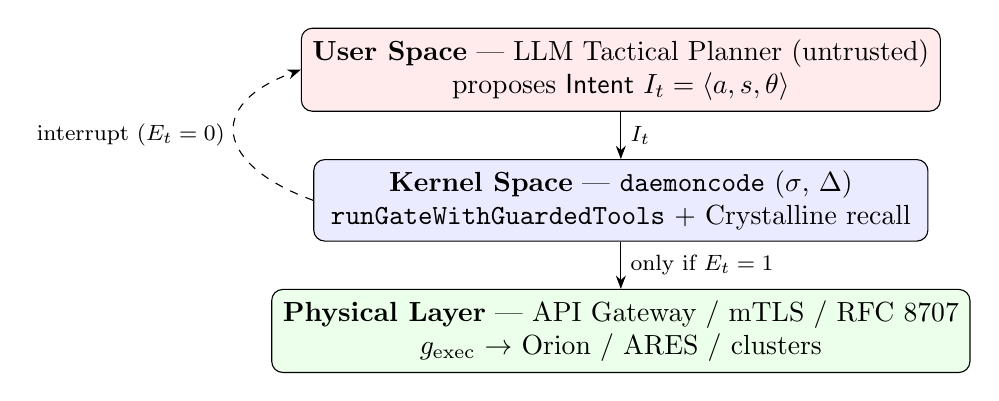
\begin{tikzpicture}[
  node distance=6mm,
  box/.style={draw,rounded corners,align=center,inner sep=4pt,minimum width=78mm},
  tier/.style={draw,dashed,rounded corners,inner sep=6pt}
]
\node[box,fill=red!8]   (llm)  {\textbf{User Space} --- LLM Tactical Planner (untrusted)\\ proposes \textsf{Intent} $I_t=\langle a,s,\theta\rangle$};
\node[box,fill=blue!8,below=of llm]  (kernel) {\textbf{Kernel Space} --- \texttt{daemoncode} ($\sigma$, $\Delta$)\\ \texttt{runGateWithGuardedTools} + Crystalline recall};
\node[box,fill=green!8,below=of kernel] (phys) {\textbf{Physical Layer} --- API Gateway / mTLS / RFC 8707\\ $g_{\text{exec}}$ $\rightarrow$ Orion / ARES / clusters};
\draw[-{Stealth}] (llm) -- node[right]{\footnotesize $I_t$} (kernel);
\draw[-{Stealth}] (kernel) -- node[right]{\footnotesize only if $E_t=1$} (phys);
\draw[-{Stealth},dashed] (kernel.west) to[out=160,in=200,looseness=2] node[left]{\footnotesize interrupt ($E_t=0$)} (llm.west);
\end{tikzpicture}
\caption{Three-tier topology. The LLM only emits proposals. The kernel decides;
a network packet ($E_t=1$) is emitted only for actions that pass the shield.
Blocked actions ($E_t=0$) are reflected back as cognitive interrupts.}
\label{fig:tiers}
\end{figure}

\section{Formal Safety Model}
\label{sec:model}
We model the system as a shielded MDP. The global state factorises as
\begin{equation}
\mathcal{S}=\mathcal{S}_{\text{code}}\times\mathcal{S}_{\text{mem}}\times
\mathcal{S}_{\text{net}}\times\mathcal{S}_{\text{gate}},
\end{equation}
covering code/artefact state, cognitive memory, network-perimeter state, and the
gate machine (including retry counters $(r_{\text{gate}},r_{\text{global}})$).
The LLM is a stochastic policy $\pi_\theta(a\mid h_t)$ over the action set
$\mathcal{A}_{\text{LLM}}=\{I=\langle a,s,\theta\rangle\}$.

\begin{definition}[Shield]
The kernel defines, for each state $s$, a set of safe actions
$\mathcal{A}_{\text{safe}}(s)\subseteq\mathcal{A}_{\text{LLM}}$ via an enforcement
predicate $f_{\text{enforce}}$ built from active \textsc{principle} memories
(\texttt{blockedActions}, \texttt{requiredSOP}) and semiotic links. The shield
operator $\sigma$ projects any proposed $a$ onto an executable action
$a_{\text{exec}}=\sigma(a,s)$; if $a\notin\mathcal{A}_{\text{safe}}(s)$ the
projection is a cognitive interrupt that leaves $\mathcal{S}_{\text{net}}$
unchanged. The realised policy is $\pi'=\sigma\circ\pi_\theta$.
\end{definition}

\begin{definition}[Safe set]
\begin{equation}
\mathcal{S}_{\text{safe}}=\{s\in\mathcal{S}\mid
s_{\text{net}}\neq\textbf{COMPROMISED}\ \wedge\
r_{\text{gate}}\le K_{\text{gate}}\}.
\end{equation}
\end{definition}

The desired global invariant is that, starting in $\mathcal{S}_{\text{safe}}$,
the system stays in $\mathcal{S}_{\text{safe}}$ under \emph{any} policy:
\begin{equation}
\forall s\in\mathcal{S}_{\text{safe}},\ \forall a\in\mathcal{A}_{\text{LLM}}:\quad
\sum_{s'\in\mathcal{S}_{\text{safe}}} P\big(s'\mid s,\sigma(a,s)\big)=1.
\label{eq:invariant}
\end{equation}

\section{The \textsc{Gate~3} Remediation Automaton}
\label{sec:gate3}
The full state is intractable to enumerate, but the safety-relevant projection
for the smart-contract remediation gate is finite. We project to
\begin{equation}
s_\delta=\langle r,\sigma_{\text{sop}}\rangle,\quad r\in\{0,1,2,3\},\
\sigma_{\text{sop}}\in\{0,1\},
\end{equation}
where $r$ tracks the local retry counter (with $K_{\text{gate}}=3$) and
$\sigma_{\text{sop}}=1$ iff a mandatory SOP scan (\texttt{ares\_scan\_directory})
has completed successfully. The simplified action alphabet is
$\{I_{\text{bad}},I_{\text{sop}},I_{\text{done}}\}$ for forbidden actions,
mandatory-SOP actions, and the completion signal. The deterministic transition
$\Delta_\delta$ is given in Table~\ref{tab:delta}.

\begin{table}[H]
\centering
\caption{Deterministic transition $\Delta_\delta$ for \textsc{Gate~3}.
$E_t$ is the physical network-emission flag.}
\label{tab:delta}
\small
\begin{tabular}{llllc}
\toprule
State $\langle r,\sigma\rangle$ & Intent & $f_{\text{enforce}}$ & Next state & $E_t$ \\
\midrule
$\langle 0,0\rangle$ & $I_{\text{bad}}$  & 1 & $\langle 1,0\rangle$ & 0 \\
$\langle 0,0\rangle$ & $I_{\text{sop}}$  & 0 & $\langle 0,1\rangle$ & 1 \\
$\langle 0,0\rangle$ & $I_{\text{done}}$ & 0 & \textbf{ROLLBACK} & 0 \\
$\langle 1,0\rangle$ & $I_{\text{bad}}$  & 1 & $\langle 2,0\rangle$ & 0 \\
$\langle 1,0\rangle$ & $I_{\text{sop}}$  & 0 & $\langle 0,1\rangle$ & 1 \\
$\langle 2,0\rangle$ & $I_{\text{bad}}$  & 1 & \textbf{ROLLBACK} ($r\ge 3$) & 0 \\
$\langle 0,1\rangle$ & $I_{\text{done}}$ & 0 & \textbf{PROCEED} & 1 \\
\bottomrule
\end{tabular}
\end{table}

\begin{theorem}[No Unsafe Network Emission]
For every turn $t$, if the proposed intent is forbidden ($I_t=I_{\text{bad}}$)
then $E_t=0$.
\end{theorem}
\begin{proof}
By Table~\ref{tab:delta}, every row whose intent is $I_{\text{bad}}$ has
$f_{\text{enforce}}=1$, which routes the transition through the interrupt branch:
the counters update and a violation is logged, but $\mathcal{S}_{\text{net}}$ is
unchanged and $E_t=0$. No other branch is reachable for $I_{\text{bad}}$, hence
$E_t=0$ in all cases. \qed
\end{proof}

\begin{theorem}[Bounded Termination]
Every \textsc{Gate~3} episode reaches a terminal state
(\textbf{PROCEED} or \textbf{ROLLBACK}) in at most
$T_{\max}=K_{\text{gate}}+1=4$ turns, for any policy $\pi_\theta$.
\end{theorem}
\begin{proof}
Each $I_{\text{bad}}$ (or an illegal $I_{\text{done}}$ with
$\sigma_{\text{sop}}=0$) strictly increments $r$. After at most $K_{\text{gate}}$
increments, $r\ge K_{\text{gate}}$ forces a \textbf{ROLLBACK}. The only way to
avoid this is an $I_{\text{sop}}$ (setting $\sigma_{\text{sop}}=1$, resetting
$r$) followed by $I_{\text{done}}$, which reaches \textbf{PROCEED}. The
\textbf{ROLLBACK} branch terminates in at most $K_{\text{gate}}=3$ turns (three
consecutive $I_{\text{bad}}$). The \textbf{PROCEED} branch is longest when an
initial blocked turn is followed by SOP execution and completion, i.e.\ one
blocked turn plus a reset run of length $K_{\text{gate}}$, bounded by
$T_{\max}=K_{\text{gate}}+1=4$. Hence every episode terminates within
$T_{\max}=4$ turns. \qed
\end{proof}

\noindent Consequently, the reachable trajectory space collapses to two terminal
orbits, $\{\tau_{\text{success}},\tau_{\text{killed}}\}$, both contained in
$\mathcal{S}_{\text{safe}}$ by Eq.~\eqref{eq:invariant}.

\section{Implementation and Trinity Fixtures}
\label{sec:impl}
The transition table is realised one-to-one by the kernel loop
\texttt{runGateWithGuardedTools}. Each turn (i) requests a proposal from the
planner, (ii) consults Crystalline for \texttt{blockedActions}, (iii) computes a
decision, (iv) delegates state mutation and logging to an atomic helper
(\texttt{applyViolationPenalty} for hard violations), and (v) emits a
\texttt{TelemetryRow}. The telemetry row instantiates the formal tuple
$\mathbf{T}_t=[\textit{gate},t,a,\textit{status},E_t]$, where the boolean
\texttt{network\_emitted} is the concrete instance of $E_t\in\{0,1\}$ and
\texttt{r\_gate}/\texttt{sigma\_sop} instantiate $r$/$\sigma_{\text{sop}}$.

\begin{lstlisting}[language=TypeScript,caption={Atomic violation helper (excerpt).}]
export function applyViolationPenalty(ctx, registers, config, recorder, history) {
  registers.r_gate++; registers.r_global++;
  const terminal = registers.r_gate >= config.maxGateRetries
                || registers.r_global >= config.maxGlobalRetries;
  const status = terminal ? "ROLLBACK" : "BLOCKED";
  recorder.record({ gate: ctx.gate, turn: ctx.turn,
    action_schema: ctx.action_schema, enforcer_status: status,
    network_emitted: false });            // I_bad => E_t = 0
  if (terminal) return { shouldBreak: true, finalStatus: "ROLLBACK" };
  history.push({ role: "tool",   content: JSON.stringify({ blocked: ctx.action_schema }) });
  history.push({ role: "system", content: ctx.interruptMessage });
  return { shouldBreak: false, finalStatus: "PENDING" };
}
\end{lstlisting}

\noindent The three \emph{Trinity Fixtures} are golden traces that pin the runtime
to $\Delta_\delta$ and are encoded as unit tests:
\begin{description}
  \item[Fixture 1 (Synonym Attack).] A stubborn planner emits
  \texttt{deploy\_to\_prod}, \texttt{force\_publish}, \texttt{trigger\_pipeline},
  \texttt{deploy\_to\_prod}. Every turn is \texttt{BLOCKED} with
  \texttt{network\_emitted=false}; the retry budget is exhausted after
  $K_{\text{gate}}=3$ increments, so the episode ends in \textbf{ROLLBACK} at
  turn 3 (Bounded Termination).
  \item[Fixture 2 (Sandbox Escape).] A planner falls back to a generic tool
  (\texttt{execute\_bash}). All turns are blocked; \textbf{ROLLBACK} at turn 3.
  \item[Fixture 3 (SOP-Compliant Path).] After one blocked
  \texttt{deploy\_to\_prod}, the planner runs \texttt{ares\_scan\_directory} and
  \texttt{ouroboros\_scan} (each \texttt{SUCCESS}, \texttt{network\_emitted=true})
  and then \texttt{complete\_gate\_task} $\rightarrow$ \textbf{PROCEED}.
\end{description}
Any change to the kernel that violates $\Delta_\delta$ is caught as a regression
failure, making the formal model an enforced contract rather than documentation.

\section{Uncertainty-Aware (Pessimistic) Shielding}
\label{sec:uncertainty}
A naive shield trusts the external scanners (ARES, ouroboros) as perfect
oracles. To remove this assumption we add a scanner-confidence variable
$\gamma_{\text{scan}}\in[0,1]$ and adopt a default-deny posture:
\begin{equation}
f_{\text{enforce}}(I_t,M)=
\begin{cases}
1, & \exists m\in M:\ I_t.a\in m.A_{\text{blocked}}\ \wedge\ \gamma_{\text{scan}}\ge\gamma_{\text{thr}}\\
1, & \gamma_{\text{scan}}<\gamma_{\text{thr}}\quad(\text{scanner uncertain})\\
0, & \text{otherwise.}
\end{cases}
\end{equation}
A false negative under low confidence no longer opens an execution path; the
agent is forced onto the SOP route or human-in-the-loop. The two \textsc{Gate~3}
theorems are preserved because the only effect of low confidence is to add more
$f_{\text{enforce}}=1$ transitions, which never emit network packets and never
extend the retry bound.

\section{Threats to Validity and Future Work}
The proofs rely on (i) the kernel and gateway faithfully implementing
$\sigma$ and $\Delta$, and (ii) the semiotic layer correctly mapping forbidden
synonyms into $I_{\text{bad}}$. New evasion tools are handled by extending the
semiotic links and \textsc{principle} memories, \emph{not} by mutating the
kernel, preserving $\mathcal{S}_{\text{safe}}$. The present validation is
design-level plus an executable regression suite; a probabilistic model checker
(e.g.\ PRISM/Storm) over the eight-state automaton and empirical ``live-fire''
logs against a real LLM are natural next steps.

\section{Conclusion}
Safety in the Daemon Protocol is a property of a deterministic kernel, not of the
LLM's disposition. By reducing the smart-contract remediation gate to a finite
shielded automaton with a bounded retry budget, we obtain two machine-checkable
safety properties and bind them to a concrete runtime via the Trinity Fixtures.
The result is a reproducible methodology for building autonomous coding agents
that may be wrong but cannot be destructive.

\end{document}
